\documentclass[a4paper,10pt]{article}
\usepackage[utf8]{inputenc}

\usepackage{tikz}
\usepackage{bbm}
\usepackage{amsmath}
\usepackage{hyperref}

\newcommand\Shifted[2]{\Delta_{#1}(#2)}
\newcommand\Reversed[1]{\overline{#1}}

\newcommand\SymSquare{\begin{tikzpicture}%
        \draw (0,0) -- (0,1em) -- (1em,1em) -- (1em,0) -- cycle;
\end{tikzpicture}}
\newcommand\Indicator[1]{\SymSquare(#1)}

\newcommand\SymPositiveTriangle{
\begin{tikzpicture}%
        \draw (0,0) -- (1em,0em) -- (1em,1em) -- cycle;
\end{tikzpicture}}
\newcommand\PositiveTriangle[1]{\SymPositiveTriangle(#1)}

\newcommand\SymNegativeTriangle{
\begin{tikzpicture}%
        \draw (0,0) -- (0,1em) -- (1em,0em) -- cycle;
\end{tikzpicture}}
\newcommand\NegativeTriangle[1]{\SymNegativeTriangle(#1)}

\newcommand\SymTrapezoid{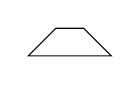
\begin{tikzpicture}%
        \draw (0,0) -- (3em,0) -- (2em,1em) -- (1em,1em) -- cycle;
\end{tikzpicture}}
\newcommand\Trapezoid[2]{\SymTrapezoid(#1,#2)}% Trapezoid(h,b)

\newcommand\D{\mathrm{d}}
\newcommand\Convolution{\star}
\newcommand\ConvolutionInt[2]{\int_{-\infty}^{\infty}#1 \D#2}
\newcommand\Equiv{\Leftrightarrow}
\newcommand\Then{\Rightarrow}
\renewcommand\And{\wedge}

% \GridAxis{from_x}{to_x}{from_y}{to_y}
\newcommand\GridAxis[4]{%
    \draw[very thin,color=gray] (#1,#3) grid (#2,#4);
    \draw[->] (#1,0) -- (#2,0) node[right] {$x$};
    \draw[->] (0,#3) -- (0,#4);
    \node[below right] at (0,0) {$0$};
    \coordinate (Origin) at (0,0);
    \coordinate (FuncStart) at (#1,0);
    \coordinate (FuncEnd) at (#2,0);
}
\newcommand\SizedGridAxis[4]{%
    \GridAxis{#1}{#2}{#3}{#4}
    \node[below right] at (0,1) {$1$};
    \node[below right] at (1,0) {$1$};
}

%%%%%%%%%%%%%%%%%%%%%%%%%%%%%%%%%%%%%%%%%%%%%%%%%%%%%%%%%%%%%%%%%%%%%%%%%%%%%%%
\title{Convolution formulas using shapes}
\author{Francois Gindraud}
\date{}
\begin{document}
\maketitle

Formulas for convolutions are very quickly unwieldy, especially if the functions being convoluted are defined by parts.
This document shows the \emph{shape} approach to convolutions: functions are decomposed into simple geometrical shapes, and convolution of the functions are defined by combining the convolutions of simple shapes.

Pros:
\begin{itemize}
    \item Manipulate only small formulas for each shape.
    \item Individual shape convolution formulas are easier to check than huge flat formulas with lots of min/max.
    \item More readable implementation of formulas into code.
    \item High level simplifications are easier to detect if some shapes cancel with others.
\end{itemize}
Cons:
\begin{itemize}
    \item Missed simplification opportunities, if the simplifications only happen between the formulas of different shapes.
    \item More verbose than the flat strategy.
\end{itemize}

\paragraph{Convolution}
Convolution is noted using the $\Convolution$ operator, with the usual definition:
\[ \left[ f \Convolution g \right](x) = \ConvolutionInt{f(x - t) g(t)}{t} \]
Convolution is commutative and associative.

%%%%%%%%%%%%%%%%%%%%%%%%%%%%%%%%%%%%%%%%%%%%%%%%%%%%%%%%%%%%%%%%%%%%%%%%%%%%%%%
\section{Combinators}

\paragraph{Time shifting}
The time shift combinator of shift $h$ moves the shape $f$ forward along the time axis by $h$.
For a shape $f$ \emph{centered} on $c$, $\Shifted{h}{f}$ is \emph{centered} on $c+h$.
\[ \Shifted{h}{f}(x) = f(x - h) \]
Time shifts combine additively:
\[ \Shifted{h}{\Shifted{h'}{f}}= \Shifted{h+h'}{f} \]
Convolution of shifted functions is the shift of convolutions:
\[
    \left[ \Shifted{h}{f} \Convolution g \right](x) =
    \ConvolutionInt{ f((x - t) - h) g(t) }{t} =
    \left[ f \Convolution g \right](x-h) =
    \Shifted{h}{f \Convolution g}(x)
\]

\paragraph{Scaling}
The scaling combinator scales the shape $f$ by a factor $c$ on the vertical axis.
\[ \left[ c \times f \right] (x) = c \times f(x) \]
Scaling combines multiplicatively with itself, and can be swapped with time shift:
\[ c \times (c' \times f) =  (c \times c') \times f \]
\[ c \times (\Shifted{h}{f}) = \Shifted{h}{c \times f} \]
Convolution of scaled functions is a scaled convolution:
\[ (c \times f) \Convolution g = c \times (f \Convolution g) \]

\paragraph{Time inversion}
A \emph{reversed} function is the shape mirrored by the vertical axis:
\[ \Reversed{f}(x) = f(-x) \]
Simplifications:
\[ \Reversed{\Reversed{f}} = f \]
\[ \Reversed{c \times f} = c \times \Reversed{f} \]
\[ \Reversed{\Shifted{h}{f}}(x) = \Shifted{h}{f}(-x) = f(-x-h) = \Reversed{f}(x+h) = \Shifted{-h}{\Reversed{f}}(x) \]
Convolution:
\[
    \Reversed{f \Convolution g}(x) = \ConvolutionInt{f(-x-t) g(t)}{t} = \ConvolutionInt{f(-x+T) g(-T)}{T} = \left[ \Reversed{f} \Convolution \Reversed{g} \right] (x)
\]

%%%%%%%%%%%%%%%%%%%%%%%%%%%%%%%%%%%%%%%%%%%%%%%%%%%%%%%%%%%%%%%%%%%%%%%%%%%%%%%
\section{Basic shapes}

\paragraph{Indicator function}
The \emph{indicator function} of width $l$ is a rectangle of width $l$, height $1$, horizontally centered on $0$.
\begin{center}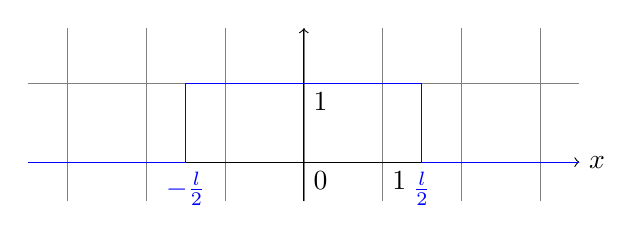
\begin{tikzpicture}
    \SizedGridAxis{-3.5}{3.5}{-0.5}{1.7}
    \begin{scope}[color=blue]
        \draw (FuncStart) -- (-1.5,0) coordinate(a) -- (-1.5,1) -- (1.5,1) -- (1.5,0) coordinate(b) -- (FuncEnd);
        \node[below] at (a) {$-\frac{l}{2}$};
        \node[below] at (b) {$\frac{l}{2}$};
    \end{scope}
\end{tikzpicture}\end{center}
\[
    \Indicator{l}(x) =
    \mathbbm{1}_{\left[ -\frac{l}{2}, \frac{l}{2} \right]}(x) =
    \begin{cases}
        1 & x \in \left[ -\frac{l}{2}, \frac{l}{2} \right] \\
        0 & \text{otherwise}
    \end{cases}
\]
The function is symmetric:
\[ \Reversed{\Indicator{l}}(x) = \Indicator{l}(-x) = \Indicator{l}(x) \]

\paragraph{Positive triangle}
The \emph{positive triangle} of side $c$ is a triangle formed by coordinates $\{ (0,0), (c, 0), (c,c) \}$:
\begin{center}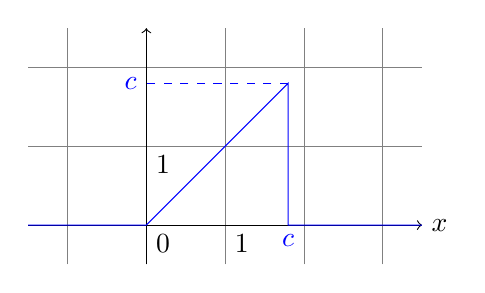
\begin{tikzpicture}
    \SizedGridAxis{-1.5}{3.5}{-0.5}{2.5}
    \begin{scope}[color=blue]
        \draw (FuncStart) -- (0,0) -- (1.8,1.8) coordinate(a) -- (1.8,0) coordinate(b) -- (FuncEnd);
        \draw[dashed] (a) -- (a -| Origin) node[left] {$c$};
        \node[below] at (b) {$c$};
    \end{scope}
\end{tikzpicture}\end{center}
\[
    \PositiveTriangle{c}(x) = \begin{cases}
        x & x \in \left[ 0, c \right] \\
        0 & \text{otherwise}
    \end{cases}
\]

\paragraph{Negative triangle}
The \emph{negative triangle} of side $c$ is a triangle formed by coordinates $\{ (0,0), (-c, 0), (-c,c) \}$:
\begin{center}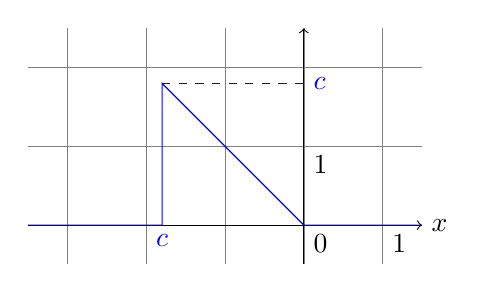
\begin{tikzpicture}
    \SizedGridAxis{-3.5}{1.5}{-0.5}{2.5}
    \begin{scope}[color=blue]
        \draw (FuncStart) -- (-1.8,0) coordinate(a) -- (-1.8,1.8) coordinate(b) -- (0,0) -- (FuncEnd);
        \draw[dashed] (b) -- (b -| Origin) node[right] {$c$};
        \node[below] at (a) {$c$};
    \end{scope}
\end{tikzpicture}\end{center}
\[
    \NegativeTriangle{c}(x) = \begin{cases}
        -x & x \in \left[ -c, 0 \right] \\
        0 & \text{otherwise}
    \end{cases}
\]
A reversed negative triangle is a positive triangle:
\[ \Reversed{\NegativeTriangle{c}}(x) =  \NegativeTriangle{c}(-x) = \PositiveTriangle{c}(x) \]

\paragraph{Trapezoid}
A \emph{trapezoid} of height $h$ and central block width $b$ is formed by a central rectangle of size $(b,h)$ centered on $0$, and flanked by triangles of side size $h$:

\begin{center}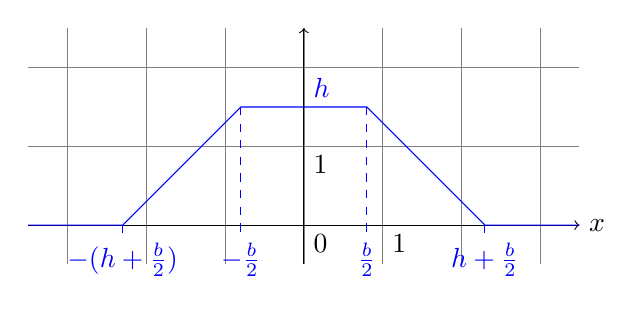
\begin{tikzpicture}
    \SizedGridAxis{-3.5}{3.5}{-0.5}{2.5}
    \begin{scope}[color=blue]
        \draw (FuncStart) -- (-2.3,0) coordinate(a) -- (-0.8,1.5) coordinate(b) -- (0.8,1.5) coordinate(c) -- (2.3,0) coordinate(d) -- (FuncEnd);
        \node[above right] at (b -| Origin) {$h$};
        \draw (a) -- ++(0,-0.1) node[below] {$-(h+\frac{b}{2})$};
        \draw[dashed] (b) -- (b |- Origin) -- +(0,-0.1) node[below] {$-\frac{b}{2}$};
        \draw[dashed] (c) -- (c |- Origin) -- +(0,-0.1) node[below] {$\frac{b}{2}$};
        \draw (d) -- ++(0,-0.1) node[below] {$h+\frac{b}{2}$};
    \end{scope}
\end{tikzpicture}\end{center}
\[
    \Trapezoid{h}{b}(x) = \begin{cases}
        x - (h + \frac{b}{2}) & x \in \left[ - (h + \frac{b}{2}), -\frac{b}{2} \right] \\
        h & x \in \left[ -\frac{b}{2}, \frac{b}{2} \right] \\
        (h + \frac{b}{2}) - x & x \in \left[ \frac{b}{2}, h + \frac{b}{2} \right] \\
        0 & \text{otherwise}
    \end{cases}
\]
A trapezoid is symetric:
\[ \Reversed{\Trapezoid{h}{b}}(x) = \Trapezoid{h}{b}(-x) = \Trapezoid{h}{b}(x) \]
A trapezoid can be decomposed into an indicator function and two triangles:
\[ \Trapezoid{h}{b} = \Shifted{-(h+\frac{b}{2})}{\PositiveTriangle{h}} + h \times \Indicator{b} + \Shifted{h+\frac{b}{2}}{\NegativeTriangle{h}} \]
A trapezoid is the resulting shape of a convolution of two rectangles (see~\ref{proof_convolution_indicator_indicator}):
\[ \Indicator{a} \Convolution \Indicator{b} = \Trapezoid{\min(a,b)}{|a - b|} \]

%%%%%%%%%%%%%%%%%%%%%%%%%%%%%%%%%%%%%%%%%%%%%%%%%%%%%%%%%%%%%%%%%%%%%%%%%%%%%%%
\section{Complex convolution shapes}

\subsection{Convolution of indicator with positive triangle}
\[ C_{l,c}(x) = \left[ \Indicator{l} \Convolution \PositiveTriangle{c} \right] (x) \]

\paragraph{Case 1}
$l \le c$.
\begin{center}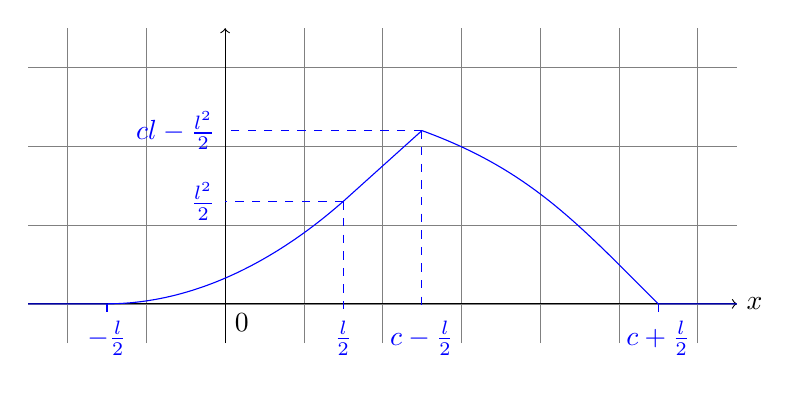
\begin{tikzpicture}
    \GridAxis{-2.5}{6.5}{-0.5}{3.5}
    \begin{scope}[color=blue]
        \draw (FuncStart) -- (-1.5,0) coordinate(a) parabola (1.5,1.3) coordinate(b) -- (2.5,2.2) coordinate(c) to[out=-20,in=135] (5.5,0) coordinate(d) -- (FuncEnd);
        \draw (a) -- +(0,-0.1) node[below] {$-\frac{l}{2}$};
        \draw[dashed] (b) -- (b |- Origin) -- +(0,-0.1) node[below] {$\frac{l}{2}$};
        \draw[dashed] (b) -- (b -| Origin) node[left] {$\frac{l^2}{2}$};
        \draw[dashed] (c) -- (c |- Origin) -- +(0,-0.1) node[below] {$c-\frac{l}{2}$};
        \draw[dashed] (c) -- (c -| Origin) node[left] {$cl-\frac{l^2}{2}$};
        \draw (d) -- +(0,-0.1) node[below] {$c+\frac{l}{2}$};
    \end{scope}
\end{tikzpicture}\end{center}
\[ C_{l,c}(x) = \begin{cases}
    0 & x \le -\frac{l}{2} \\
    \frac{1}{2} (x+\frac{l}{2})^2 & x \in \left[ -\frac{l}{2}, \frac{l}{2} \right] \\
    xl & x \in \left[ \frac{l}{2}, c-\frac{l}{2} \right] \\
    \frac{1}{2} (c^2 - (x-\frac{l}{2})^2) & x \in \left[ c-\frac{l}{2}, c+\frac{l}{2} \right] \\
    0 & x \ge c+\frac{l}{2}
\end{cases} \]
Slopes :
\[ \left. \frac{\D(\frac{1}{2} (x+\frac{l}{2})^2)}{\D x} \right|_{x=-\frac{l}{2}} = 0 \]
\[ \left. \frac{\D(\frac{1}{2} (x+\frac{l}{2})^2)}{\D x} \right|_{x=\frac{l}{2}} = l = \left. \frac{\D(xl)}{\D x} \right|_{x=\frac{l}{2}} \]
\[ \left. \frac{\D(\frac{1}{2} (c^2 - (x-\frac{l}{2})^2))}{\D x} \right|_{x=c-\frac{l}{2}} = l - c \le 0 \]

\paragraph{Case 2}
$l \ge c$
\begin{center}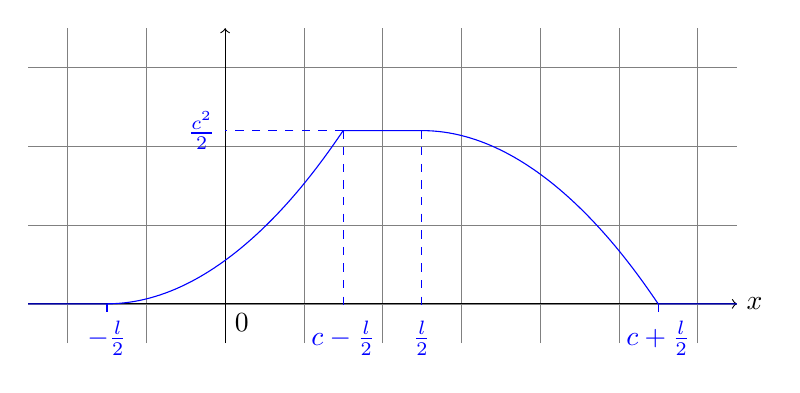
\begin{tikzpicture}
    \GridAxis{-2.5}{6.5}{-0.5}{3.5}
    \begin{scope}[color=blue]
        \draw (FuncStart) -- (-1.5,0) coordinate(a) parabola (1.5,2.2) coordinate(b) -- (2.5,2.2) coordinate(c) parabola (5.5,0) coordinate(d) -- (FuncEnd);
        \draw (a) -- +(0,-0.1) node[below] {$-\frac{l}{2}$};
        \draw[dashed] (b) -- (b |- Origin) -- +(0,-0.1) node[below] {$c-\frac{l}{2}$};
        \draw[dashed] (b) -- (b -| Origin) node[left] {$\frac{c^2}{2}$};
        \draw[dashed] (c) -- (c |- Origin) -- +(0,-0.1) node[below] {$\frac{l}{2}$};
        \draw (d) -- +(0,-0.1) node[below] {$c+\frac{l}{2}$};
    \end{scope}
\end{tikzpicture}\end{center}
\[ C_{l,c}(x) = \begin{cases}
    0 & x \le -\frac{l}{2} \\
    \frac{1}{2} (x+\frac{l}{2})^2 & x \in \left[ -\frac{l}{2}, c-\frac{l}{2} \right] \\
    \frac{c^2}{2} & x \in \left[ c-\frac{l}{2}, \frac{l}{2} \right] \\
    \frac{1}{2} (c^2 - (x-\frac{l}{2})^2) & x \in \left[ \frac{l}{2}, c+\frac{l}{2} \right] \\
    0 & x \ge c+\frac{l}{2}
\end{cases} \]
Slopes:
\[ \left. \frac{\D(\frac{1}{2} (c^2 - (x-\frac{l}{2})^2))}{\D x} \right|_{x=\frac{l}{2}} = 0 \]

\paragraph{Factorized}
By posing $(a,b) = (\min(\frac{l}{2}, c-\frac{l}{2}), \max(\frac{l}{2}, c-\frac{l}{2}))$, we can use a condensed form for the convolution:
\[ C_{l,c}(x) = \begin{cases}
    0 & x \le -\frac{l}{2} \\
    \frac{1}{2} (x+\frac{l}{2})^2 & x \in \left[ -\frac{l}{2}, a \right] \\
    xl & x \in \left[ a, b \right] \And l \le c \\
    \frac{c^2}{2} & x \in \left[ a, b \right] \And l \ge c \\
    \frac{1}{2} (c^2 - (x-\frac{l}{2})^2) & x \in \left[ b, c+\frac{l}{2} \right] \\
    0 & x \ge c+\frac{l}{2}
\end{cases} \]

Proof is in section~\ref{proof_convolution_indicator_triangle}.
Convolution with a negative triangle is obtained using time inversion:
\[
    \Indicator{l} \Convolution \NegativeTriangle{c} =
    \Reversed{\Indicator{l}} \Convolution \Reversed{\PositiveTriangle{c}} =
    \Reversed{\Indicator{l} \Convolution \PositiveTriangle{c}}
\]

\subsection{Convolution of positive triangle with positive triangle}
\[ C_{a,b}(x) = \left[ \PositiveTriangle{a} \Convolution \PositiveTriangle{b} \right] (x) \]

\paragraph{Case 1}
$a \le b$:
\begin{center}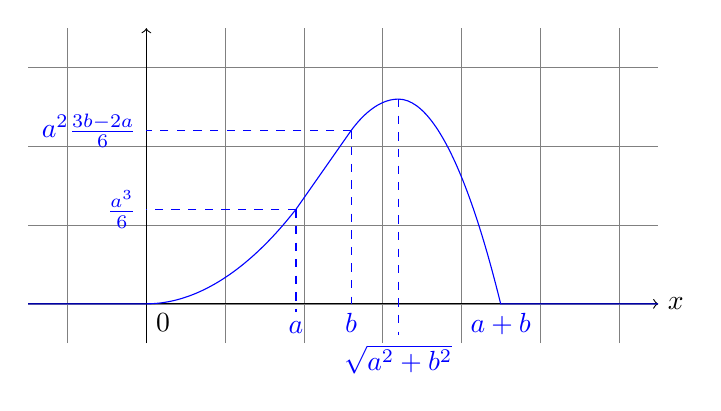
\begin{tikzpicture}
    \GridAxis{-1.5}{6.5}{-0.5}{3.5}
    \begin{scope}[color=blue]
        \draw (FuncStart) -- (Origin) parabola (1.9,1.2) coordinate(a) -- (2.6,2.2) coordinate(b) parabola bend (3.2,2.6) (4.5,0) coordinate(d) -- (FuncEnd);
        \draw[dashed] (a) -- (a |- Origin) -- +(0,-0.1) node[below] {$a$};
        \draw[dashed] (a) -- (a -| Origin) node[left] {$\frac{a^3}{6}$};
        \draw[dashed] (b) -- (b |- Origin) node[below] {$b$};
        \draw[dashed] (b) -- (b -| Origin) node[left] {$a^2 \frac{3b-2a}{6}$};
        \draw[dashed] (3.2,2.6) -- (3.2,-0.4) node[below] {$\sqrt{a^2+b^2}$};
        \node[below] at (d) {$a+b$};
    \end{scope}
\end{tikzpicture}\end{center}
\[ C_{a,b}(x) = \begin{cases}
    0 & x \le 0 \\
    \frac{x^3}{6} & x \in [0, a] \\
    a^2 \frac{3x-2a}{6} & x \in [a, b] \\
    \frac{1}{6} (a+b-x) (x^2 + x(a+b) -2a^2-2b^2+2ab) & x \in [b, a+b] \\
    0 & x \ge a+b
\end{cases} \]

Slope of $4$-th component:
\[ \frac{\D C_{a,b}^4(x)}{\D x} = \frac{\D(\frac{1}{6} (a+b-x) (x^2 + x(a+b) -2a^2-2b^2+2ab))}{\D x} = \frac{1}{2} (a^2+b^2-x^2) \]
Slopes:
\[ \left. \frac{\D(\frac{x^3}{6})}{\D x} \right|_{x=0} = 0 \]
\[
    \frac{a^2}{2} =
    \left. \frac{\D(\frac{x^3}{6})}{\D x} \right|_{x\in [a,b]} =
    \left. \frac{\D(a^2 \frac{3x-2a}{6})}{\D x} \right|_{x=a} =
    \left. \frac{\D C_{a,b}^4(x)}{\D x} \right|_{x=b}
\]
\[ \left. \frac{\D C_{a,b}^4(x)}{\D x} \right|_{x=\sqrt{a^2+b^2}} = 0 \]

\paragraph{Case 2}
$a \ge b$.
$C_{a,b}(x) = C_{b,a}(x)$, so this is the same shape and formula as case 1 with a swap of $a$ and $b$.

\paragraph{Factorized}
By posing $A=\min(a,b)$ and $B=\max(a,b)$ we have the condensed formula:
\[ C_{a,b}(x) = \begin{cases}
    0 & x \le 0 \\
    \frac{x^3}{6} & x \in [0, A] \\
    A^2 \frac{3x-2A}{6} & x \in [A, B] \\
    \frac{1}{6} (a+b-x) (x^2 + x(a+b) -2a^2-2b^2+2ab) & x \in [B, a+b] \\
    0 & x \ge a+b
\end{cases} \]

Proof in section~\ref{proof_convolution_triangle_pos_pos}.
Convolution with of negative triangles is obtained using time inversion:
\[
    \NegativeTriangle{a} \Convolution \NegativeTriangle{b} =
    \Reversed{\PositiveTriangle{a}} \Convolution \Reversed{\PositiveTriangle{b}} =
    \Reversed{\PositiveTriangle{a} \Convolution \PositiveTriangle{b}}
\]

%%%%%%%%%%%%%%%%%%%%%%%%%%%%%%%%%%%%%%%%%%%%%%%%%%%%%%%%%%%%%%%%%%%%%%%%%%%%%%%
\section{Proofs}

%%%%%%%%%%%%%%%%%%%%%%%%%%%%%%%%%%%%%%%%%%%%%%%%%%%%%%%%%%%%%%%%%%%%%%%%%%%%%%%
\subsection{Convolution of indicator with indicator}\label{proof_convolution_indicator_indicator}

We want to compute the formula for:
\[ \begin{split}
    C_{a,b}(x) = \left[ \Indicator{a} \Convolution \Indicator{b} \right] (x) & = \ConvolutionInt{\Indicator{a}(x-t) \Indicator{b}(t)}{t} \\
    & = \ConvolutionInt{\Indicator{a}(t-x) \Indicator{b}(t)}{t} \\
    & = \ConvolutionInt{\Shifted{x}{\Indicator{a}}(t) \Indicator{b}(t)}{t}
\end{split} \]
$C_{a,b}(x)$ is symmetric:
\[
    \Reversed{\Indicator{a} \Convolution \Indicator{b}} =
    \Reversed{\Indicator{a}} \Convolution \Reversed{\Indicator{b}} =
    \Indicator{a} \Convolution \Indicator{b}
\]
By using the commutativity of the convolution, $C_{a,b}(x) = C_{\min(a,b),\max(a,b)}(x)$.
Thus we can compute $C_{a,b}(x)$ for only $x \ge 0$ and $a \le b$, and extend to the whole domain using symmetries.
$C_{a,b}(x)$ is the width of the intersection between two rectangles: one of width $b$ centered on $0$, the other of width $a$ centered on $x$.
In the following pictures $\Indicator{a}$ is in red and $\Indicator{b}$ is in blue.

\paragraph{No overlap}
$x - \frac{a}{2} \ge \frac{b}{2} \Equiv x \ge \frac{a+b}{2}$.
$C_{a,b}(x) = 0$.
\begin{center}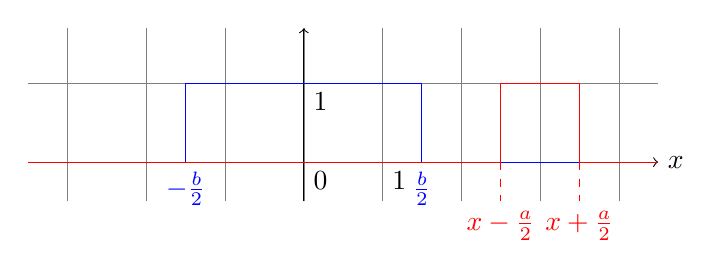
\begin{tikzpicture}
    \SizedGridAxis{-3.5}{4.5}{-0.5}{1.7}
    \begin{scope}[color=blue] % B
        \draw (FuncStart) -- (-1.5,0) coordinate(a) -- (-1.5,1) -- (1.5,1) -- (1.5,0) coordinate(b) --(FuncEnd);
        \node[below] at (a) {$-\frac{b}{2}$};
        \node[below] at (b) {$\frac{b}{2}$};
    \end{scope}
    \begin{scope}[color=red] % A
        \draw (FuncStart) -- (2.5,0) coordinate(a) -- (2.5,1) -- (3.5,1) -- (3.5,0) coordinate(b) -- (FuncEnd);
        \draw[dashed] (a) -- +(0,-0.5) node[below] {$x-\frac{a}{2}$};
        \draw[dashed] (b) -- +(0,-0.5) node[below] {$x+\frac{a}{2}$};
    \end{scope}
\end{tikzpicture}\end{center}

\paragraph{Partial overlap}
$x - \frac{a}{2} \le \frac{b}{2} \le x + \frac{a}{2} \Equiv x \in \left[ \frac{b-a}{2}, \frac{a+b}{2} \right]$.
\begin{center}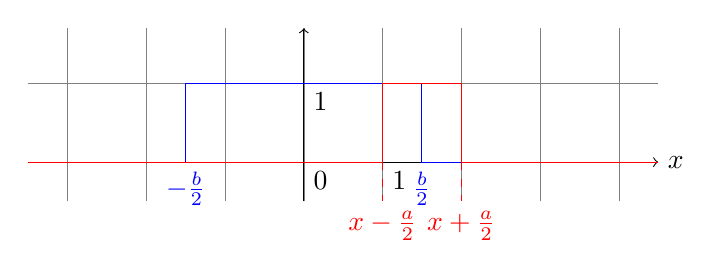
\begin{tikzpicture}
    \SizedGridAxis{-3.5}{4.5}{-0.5}{1.7}
    \begin{scope}[color=blue] % B
        \draw (FuncStart) -- (-1.5,0) coordinate(a) -- (-1.5,1) -- (1.5,1) -- (1.5,0) coordinate(b) -- (FuncEnd);
        \node[below] at (a) {$-\frac{b}{2}$};
        \node[below] at (b) {$\frac{b}{2}$};
    \end{scope}
    \begin{scope}[color=red] % A
        \draw (FuncStart) -- (1,0) coordinate(a) -- (1,1) -- (2,1) -- (2,0) coordinate(b) -- (FuncEnd);
        \draw[dashed] (a) -- +(0,-0.5) node[below] {$x-\frac{a}{2}$};
        \draw[dashed] (b) -- +(0,-0.5) node[below] {$x+\frac{a}{2}$};
    \end{scope}
\end{tikzpicture}\end{center}
\[
    C_{a,b}(x) =
    \int_{x-\frac{a}{2}}^{\frac{b}{2}} 1 \mathrm{d}t =
    \frac{b}{2} - (x - \frac{a}{2}) =
    \frac{a+b}{2} - x
\]

\paragraph{Complete inclusion}
$0 \le x \And x + \frac{a}{2} \le \frac{b}{2} \Equiv x \in \left[ 0, \frac{b-a}{2} \right] $
\begin{center}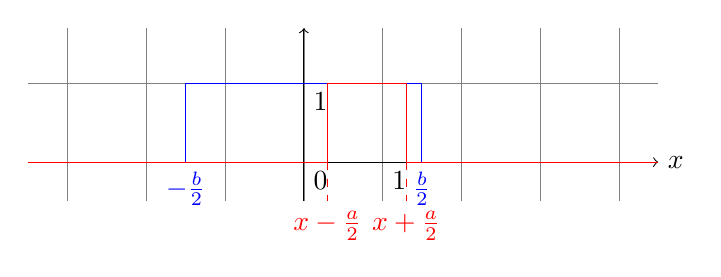
\begin{tikzpicture}
    \SizedGridAxis{-3.5}{4.5}{-0.5}{1.7}
    \begin{scope}[color=blue] % B
        \draw (FuncStart) -- (-1.5,0) coordinate(a) -- (-1.5,1) -- (1.5,1) -- (1.5,0) coordinate(b) -- (FuncEnd);
        \node[below] at (a) {$-\frac{b}{2}$};
        \node[below] at (b) {$\frac{b}{2}$};
    \end{scope}
    \begin{scope}[color=red] % A
        \draw (FuncStart) -- (0.3,0) coordinate(a) -- (0.3,1) -- (1.3,1) -- (1.3,0) coordinate(b) -- (FuncEnd);
        \draw[dashed] (a) -- +(0,-0.5) node[below] {$x-\frac{a}{2}$};
        \draw[dashed] (b) -- +(0,-0.5) node[below] {$x+\frac{a}{2}$};
    \end{scope}
\end{tikzpicture}\end{center}
\[ C_{a,b}(x) = \int_{x-\frac{a}{2}}^{x+\frac{a}{2}} 1 \mathrm{d}t = a \]

If we summarize, for $x \ge 0$ and $a \le b$:
\[ C_{a,b}(x) = \begin{cases}
    a & x \in \left[ 0, \frac{b-a}{2} \right] \\
    \frac{a+b}{2} - x & x \in \left[ \frac{b-a}{2}, \frac{a+b}{2} \right] \\
    0 & x \ge \frac{a+b}{2}
\end{cases} \]

For any $x$, $a$ and $b$, using the following identities:
\[ \min(a,b) + \max(a,b) = a + b \]
\[ \max(a,b) - \min(a,b) = |a - b| \]
\[ C_{a,b}(x) = C_{\min(a,b),\max(a,b)}(|x|) = \begin{cases}
    \min(a,b) & |x| \in \left[0, \frac{|a-b|}{2} \right] \\
    \frac{a+b}{2} - |x| & |x| \in \left[ \frac{|a-b|}{2}, \frac{a+b}{2} \right] \\
    0 & |x| \ge \frac{a+b}{2}
\end{cases} \]

By using $h = \min(a,b)$ and $l = |a-b|$, $a+b=2h+l$ and:
\[ C_{a,b}(x) = \begin{cases}
    h & |x| \in \left[0, \frac{l}{2} \right] \\
    h+\frac{l}{2} - |x| & |x| \in \left[ \frac{l}{2}, h+\frac{l}{2} \right] \\
    0 & |x| \ge h+\frac{l}{2}
\end{cases} = \Trapezoid{h}{l}(|x|) = \Trapezoid{h}{l}(x) \]

%%%%%%%%%%%%%%%%%%%%%%%%%%%%%%%%%%%%%%%%%%%%%%%%%%%%%%%%%%%%%%%%%%%%%%%%%%%%%%%
\subsection{Convolution of indicator with positive triangle}\label{proof_convolution_indicator_triangle}
\[ \begin{split}
    C_{l,c}(x) = \left[ \Indicator{l} \Convolution \PositiveTriangle{c} \right] (x) & = \ConvolutionInt{\Indicator{l}(x-t) \PositiveTriangle{c}(t)}{t} \\
    & = \ConvolutionInt{\Indicator{l}(t-x) \PositiveTriangle{c}(t)}{t} \\
    & = \ConvolutionInt{\Shifted{x}{\Indicator{l}}(t) \PositiveTriangle{c}(t)}{t}
\end{split} \]
Thus the convolution value is the area of the product between a rectangle centered on $x$ and a positive triangle with origin $0$.
In the following pictures $\Indicator{l}$ is in red and $\PositiveTriangle{c}$ is in blue.

\subsubsection{Rectangle is smaller than triangle}
$l \le c$.

\paragraph{No overlap, left}
$x+\frac{l}{2} \le 0 \Equiv x \le -\frac{l}{2}$.
$C_{l,c}(x) = 0$.
\begin{center}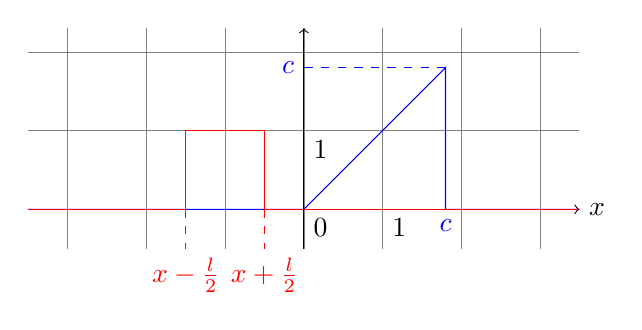
\begin{tikzpicture}
    \SizedGridAxis{-3.5}{3.5}{-0.5}{2.3}
    \begin{scope}[color=blue] % B
        \draw (FuncStart) -- (0,0) -- (1.8,1.8) coordinate(a) |- (FuncEnd);
        \node[below] at (a |- Origin) {$c$};
        \draw[dashed] (a) -- (a -| Origin) node[left] {$c$};
    \end{scope}
    \begin{scope}[color=red] % A
        \draw (FuncStart) -- (-1.5,0) coordinate(a) -- +(0,1) -- +(1,1) -- +(1,0) coordinate(b) -- (FuncEnd);
        \draw[dashed] (a) -- +(0,-0.5) node[below] {$x-\frac{l}{2}$};
        \draw[dashed] (b) -- +(0,-0.5) node[below] {$x+\frac{l}{2}$};
    \end{scope}
\end{tikzpicture}\end{center}

\paragraph{Partial left overlap}
$x+\frac{l}{2} \ge 0 \And x-\frac{l}{2} \le 0 \Equiv x \in \left[ -\frac{l}{2}, \frac{l}{2} \right]$.
\begin{center}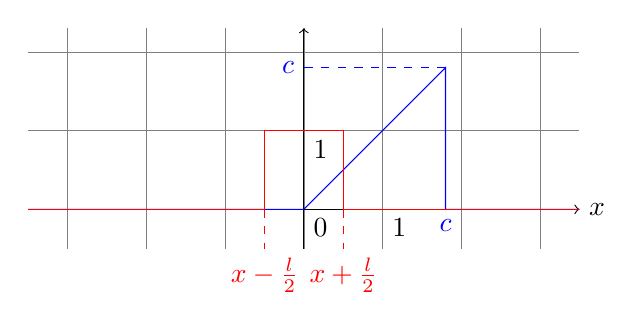
\begin{tikzpicture}
    \SizedGridAxis{-3.5}{3.5}{-0.5}{2.3}
    \begin{scope}[color=blue] % B
        \draw (FuncStart) -- (0,0) -- (1.8,1.8) coordinate(a) |- (FuncEnd);
        \node[below] at (a |- Origin) {$c$};
        \draw[dashed] (a) -- (a -| Origin) node[left] {$c$};
    \end{scope}
    \begin{scope}[color=red] % A
        \draw (FuncStart) -- (-0.5,0) coordinate(a) -- +(0,1) -- +(1,1) -- +(1,0) coordinate(b) -- (FuncEnd);
        \draw[dashed] (a) -- +(0,-0.5) node[below] {$x-\frac{l}{2}$};
        \draw[dashed] (b) -- +(0,-0.5) node[below] {$x+\frac{l}{2}$};
    \end{scope}
\end{tikzpicture}\end{center}
\[
    C_{l,c}(x) =
    \int_0^{x+\frac{l}{2}} 1 \times t \times \D t =
    \left[  \frac{t^2}{2} \right]_0^{x+\frac{l}{2}} =
    \frac{1}{2} (x+\frac{l}{2})^2
\]

\paragraph{Complete inclusion}
$x-\frac{l}{2} \ge 0 \And x+\frac{l}{2} \le c \Equiv x \in \left[ \frac{l}{2}, c-\frac{l}{2} \right]$.
\begin{center}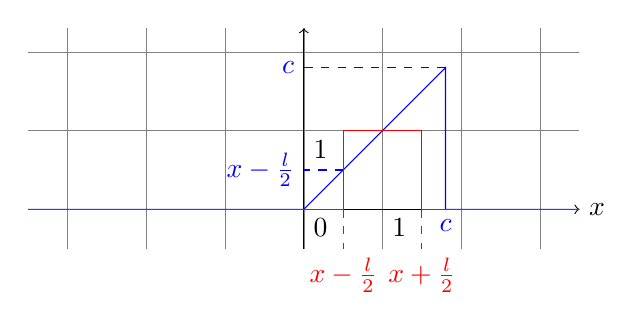
\begin{tikzpicture}
    \SizedGridAxis{-3.5}{3.5}{-0.5}{2.3}
    \begin{scope}[color=blue] % B
        \draw (FuncStart) -- (0,0) -- (1.8,1.8) coordinate(a) |- (FuncEnd);
        \node[below] at (a |- Origin) {$c$};
        \draw[dashed] (a) -- (a -| Origin) node[left] {$c$};
        \draw[dashed] (0.5,0.5) -- (0,0.5) node[left] {$x-\frac{l}{2}$};
    \end{scope}
    \begin{scope}[color=red] % A
        \draw (FuncStart) -- (0.5,0) coordinate(a) -- +(0,1) -- +(1,1) -- +(1,0) coordinate(b) -- (FuncEnd);
        \draw[dashed] (a) -- +(0,-0.5) node[below] {$x-\frac{l}{2}$};
        \draw[dashed] (b) -- +(0,-0.5) node[below] {$x+\frac{l}{2}$};
    \end{scope}
\end{tikzpicture}\end{center}
\[
    C_{l,c}(x) =
    \int_0^l 1 \times (t+x-\frac{l}{2}) \D t =
    \left[  \frac{t^2}{2}+t(x-\frac{l}{2}) \right]_0^l =
    xl
\]

\paragraph{Partial right overlap}
$x-\frac{l}{2} \le c \And x+\frac{l}{2} \ge c \Equiv x \in \left[ c-\frac{l}{2}, c+\frac{l}{2} \right]$.
\begin{center}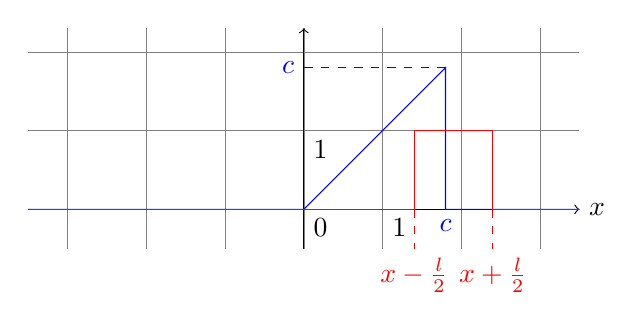
\begin{tikzpicture}
    \SizedGridAxis{-3.5}{3.5}{-0.5}{2.3}
    \begin{scope}[color=blue] % B
        \draw (FuncStart) -- (0,0) -- (1.8,1.8) coordinate(a) |- (FuncEnd);
        \node[below] at (a |- Origin) {$c$};
        \draw[dashed] (a) -- (a -| Origin) node[left] {$c$};
    \end{scope}
    \begin{scope}[color=red] % A
        \draw (FuncStart) -- (1.4,0) coordinate(a) -- +(0,1) -- +(1,1) -- +(1,0) coordinate(b) -- (FuncEnd);
        \draw[dashed] (a) -- +(0,-0.5) node[below] {$x-\frac{l}{2}$};
        \draw[dashed] (b) -- +(0,-0.5) node[below] {$x+\frac{l}{2}$};
    \end{scope}
\end{tikzpicture}\end{center}
\[
    C_{l,c}(x) =
    \int_{x-\frac{l}{2}}^c 1 \times t \times \D t =
    \left[  \frac{t^2}{2} \right]_{x-\frac{l}{2}}^c =
    \frac{1}{2} (c^2 - (x-\frac{l}{2})^2)
\]

\paragraph{No overlap, right}
$x-\frac{l}{2} \ge c \Equiv x \ge c+\frac{l}{2}$.
$C_{l,c}(x) = 0$.
\begin{center}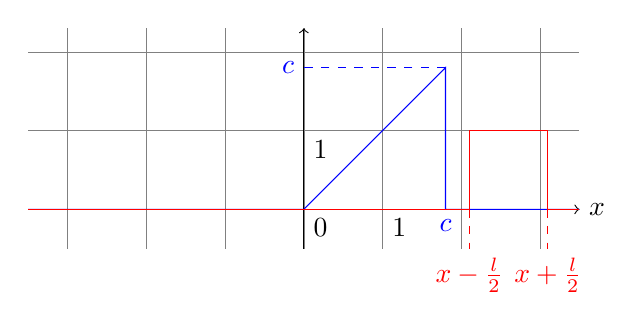
\begin{tikzpicture}
    \SizedGridAxis{-3.5}{3.5}{-0.5}{2.3}
    \begin{scope}[color=blue] % B
        \draw (FuncStart) -- (0,0) -- (1.8,1.8) coordinate(a) |- (FuncEnd);
        \node[below] at (a |- Origin) {$c$};
        \draw[dashed] (a) -- (a -| Origin) node[left] {$c$};
    \end{scope}
    \begin{scope}[color=red] % A
        \draw (FuncStart) -- (2.1,0) coordinate(a) -- +(0,1) -- +(1,1) -- +(1,0) coordinate(b) -- (FuncEnd);
        \draw[dashed] (a) -- +(0,-0.5) node[below] {$x-\frac{l}{2}$};
        \draw[dashed] (b) -- +(0,-0.5) node[below] {$x+\frac{l}{2}$};
    \end{scope}
\end{tikzpicture}\end{center}

\subsubsection{Rectangle is bigger than triangle}
$l \ge c$.

\paragraph{No overlap, left}
$x+\frac{l}{2} \le 0 \Equiv x \le -\frac{l}{2}$.
$C_{l,c}(x) = 0$.
\begin{center}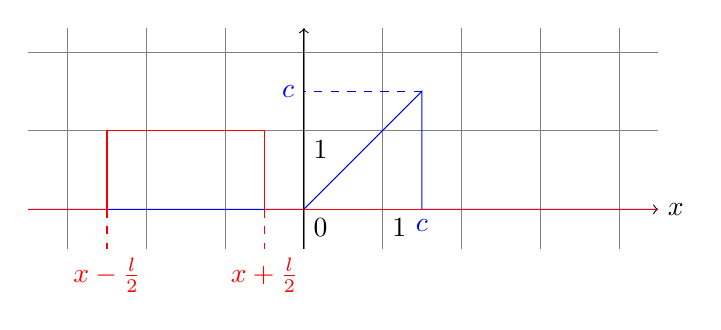
\begin{tikzpicture}
    \SizedGridAxis{-3.5}{4.5}{-0.5}{2.3}
    \begin{scope}[color=blue] % B
        \draw (FuncStart) -- (0,0) -- (1.5,1.5) coordinate(a) |- (FuncEnd);
        \node[below] at (a |- Origin) {$c$};
        \draw[dashed] (a) -- (a -| Origin) node[left] {$c$};
    \end{scope}
    \begin{scope}[color=red] % A
        \draw (FuncStart) -- (-2.5,0) coordinate(a) -- +(0,1) -- +(2,1) -- +(2,0) coordinate(b) -- (FuncEnd);
        \draw[dashed] (a) -- +(0,-0.5) node[below] {$x-\frac{l}{2}$};
        \draw[dashed] (b) -- +(0,-0.5) node[below] {$x+\frac{l}{2}$};
    \end{scope}
\end{tikzpicture}\end{center}

\paragraph{Partial left overlap}
$x+\frac{l}{2} \ge 0 \And x+\frac{l}{2} \le c \Equiv x \in \left[ -\frac{l}{2}, c-\frac{l}{2} \right]$.
\begin{center}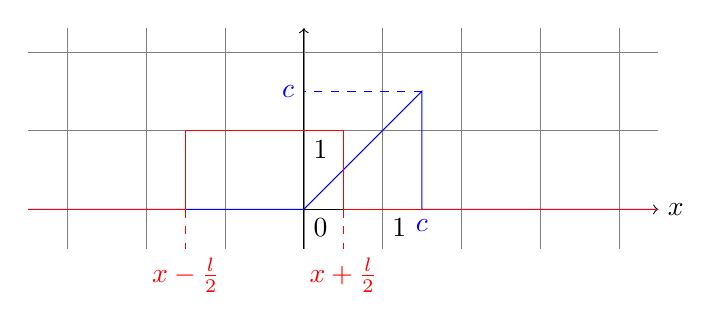
\begin{tikzpicture}
    \SizedGridAxis{-3.5}{4.5}{-0.5}{2.3}
    \begin{scope}[color=blue] % B
        \draw (FuncStart) -- (0,0) -- (1.5,1.5) coordinate(a) |- (FuncEnd);
        \node[below] at (a |- Origin) {$c$};
        \draw[dashed] (a) -- (a -| Origin) node[left] {$c$};
    \end{scope}
    \begin{scope}[color=red] % A
        \draw (FuncStart) -- (-1.5,0) coordinate(a) -- +(0,1) -- +(2,1) -- +(2,0) coordinate(b) -- (FuncEnd);
        \draw[dashed] (a) -- +(0,-0.5) node[below] {$x-\frac{l}{2}$};
        \draw[dashed] (b) -- +(0,-0.5) node[below] {$x+\frac{l}{2}$};
    \end{scope}
\end{tikzpicture}\end{center}
\[
    C_{l,c}(x) =
    \int_0^{x+\frac{l}{2}} 1 \times t \times \D t =
    \left[  \frac{t^2}{2} \right]_0^{x+\frac{l}{2}} =
    \frac{1}{2} (x+\frac{l}{2})^2
\]

\paragraph{Complete inclusion}
$x-\frac{l}{2} \le 0 \And x+\frac{l}{2} \ge c \Equiv x \in \left[ c-\frac{l}{2}, \frac{l}{2} \right]$.
\begin{center}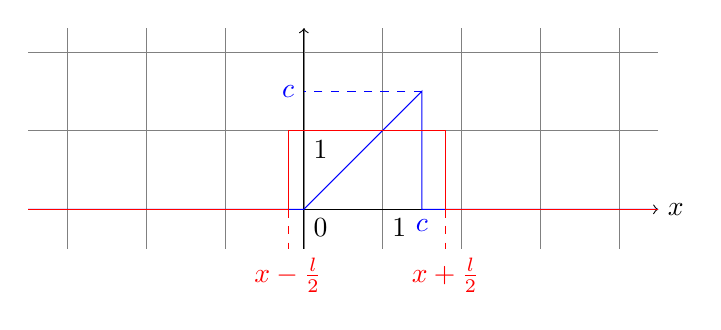
\begin{tikzpicture}
    \SizedGridAxis{-3.5}{4.5}{-0.5}{2.3}
    \begin{scope}[color=blue] % B
        \draw (FuncStart) -- (0,0) -- (1.5,1.5) coordinate(a) |- (FuncEnd);
        \node[below] at (a |- Origin) {$c$};
        \draw[dashed] (a) -- (a -| Origin) node[left] {$c$};
    \end{scope}
    \begin{scope}[color=red] % A
        \draw (FuncStart) -- (-0.2,0) coordinate(a) -- +(0,1) -- +(2,1) -- +(2,0) coordinate(b) -- (FuncEnd);
        \draw[dashed] (a) -- +(0,-0.5) node[below] {$x-\frac{l}{2}$};
        \draw[dashed] (b) -- +(0,-0.5) node[below] {$x+\frac{l}{2}$};
    \end{scope}
\end{tikzpicture}\end{center}
\[
    C_{l,c}(x) =
    \int_0^c 1 \times t \times \D t =
    \left[  \frac{t^2}{2} \right]_0^c =
    \frac{c^2}{2}
\]

\paragraph{Partial right overlap}
$0 \le x-\frac{l}{2} \le c \Equiv x \in \left[ \frac{l}{2}, c+\frac{l}{2} \right]$.
\begin{center}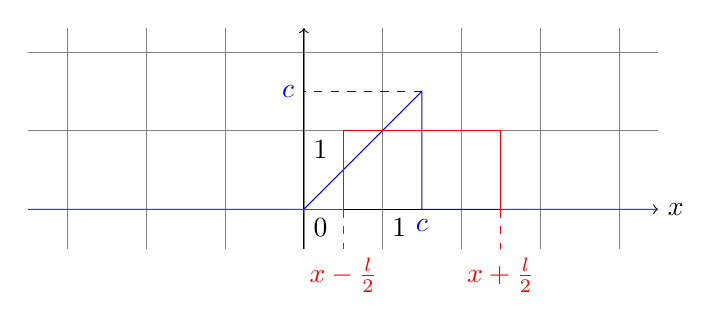
\begin{tikzpicture}
    \SizedGridAxis{-3.5}{4.5}{-0.5}{2.3}
    \begin{scope}[color=blue] % B
        \draw (FuncStart) -- (0,0) -- (1.5,1.5) coordinate(a) |- (FuncEnd);
        \node[below] at (a |- Origin) {$c$};
        \draw[dashed] (a) -- (a -| Origin) node[left] {$c$};
    \end{scope}
    \begin{scope}[color=red] % A
        \draw (FuncStart) -- (0.5,0) coordinate(a) -- +(0,1) -- +(2,1) -- +(2,0) coordinate(b) -- (FuncEnd);
        \draw[dashed] (a) -- +(0,-0.5) node[below] {$x-\frac{l}{2}$};
        \draw[dashed] (b) -- +(0,-0.5) node[below] {$x+\frac{l}{2}$};
    \end{scope}
\end{tikzpicture}\end{center}
\[
    C_{l,c}(x) =
    \int_{x-\frac{l}{2}}^c 1 \times t \times \D t =
    \left[  \frac{t^2}{2} \right]_{x-\frac{l}{2}}^c =
    \frac{1}{2} (c^2 - (x-\frac{l}{2})^2)
\]

\paragraph{No overlap, right}
$x-\frac{l}{2} \ge c \Equiv x \ge c+\frac{l}{2}$.
$C_{l,c}(x) = 0$.
\begin{center}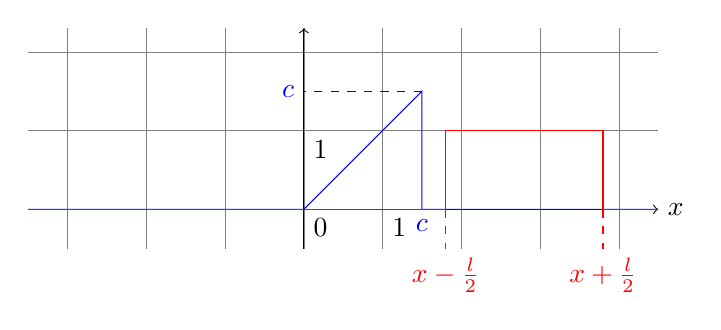
\begin{tikzpicture}
    \SizedGridAxis{-3.5}{4.5}{-0.5}{2.3}
    \begin{scope}[color=blue] % B
        \draw (FuncStart) -- (0,0) -- (1.5,1.5) coordinate(a) |- (FuncEnd);
        \node[below] at (a |- Origin) {$c$};
        \draw[dashed] (a) -- (a -| Origin) node[left] {$c$};
    \end{scope}
    \begin{scope}[color=red] % A
        \draw (FuncStart) -- (1.8,0) coordinate(a) -- +(0,1) -- +(2,1) -- +(2,0) coordinate(b) -- (FuncEnd);
        \draw[dashed] (a) -- +(0,-0.5) node[below] {$x-\frac{l}{2}$};
        \draw[dashed] (b) -- +(0,-0.5) node[below] {$x+\frac{l}{2}$};
    \end{scope}
\end{tikzpicture}\end{center}

%%%%%%%%%%%%%%%%%%%%%%%%%%%%%%%%%%%%%%%%%%%%%%%%%%%%%%%%%%%%%%%%%%%%%%%%%%%%%%%
\subsection{Convolution of positive triangle with positive triangle}\label{proof_convolution_triangle_pos_pos}
\[ \begin{split}
    C_{a,b}(x) = \left[ \PositiveTriangle{a} \Convolution \PositiveTriangle{b} \right] (x) & = \ConvolutionInt{\PositiveTriangle{a}(x-t) \PositiveTriangle{b}(t)}{t} \\
    & = \ConvolutionInt{\NegativeTriangle{a}(t-x) \PositiveTriangle{b}(t)}{t} \\
    & = \ConvolutionInt{\Shifted{x}{\NegativeTriangle{a}}(t) \PositiveTriangle{b}(t)}{t}
\end{split} \]
By using the commutativity of the convolution, $C_{a,b}(x) = C_{\min(a,b),\max(a,b)}(x)$.
Thus we can compute $C_{a,b}(x)$ for only $a \le b$, and extend to the whole domain using symmetry.
The convolution value is the area of the product between a negative triangle of origin $x$ and a positive triangle with origin $0$.
In the following pictures $\NegativeTriangle{a}$ is in red and $\PositiveTriangle{b}$ is in blue.

\paragraph{No overlap, left}
$x \le 0$.
$C_{a,b}(x) = 0$.
\begin{center}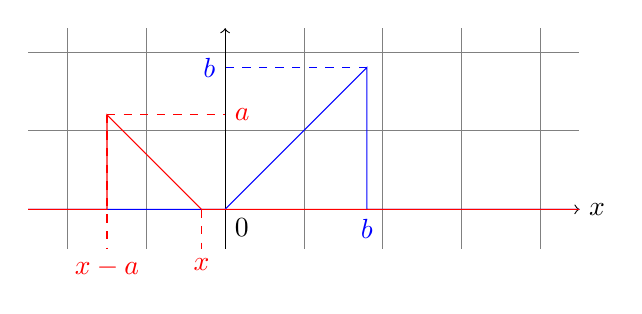
\begin{tikzpicture}
    \GridAxis{-2.5}{4.5}{-0.5}{2.3}
    \begin{scope}[color=blue] % B
        \draw (FuncStart) -- (0,0) -- (1.8,1.8) coordinate(a) |- (FuncEnd);
        \node[below] at (a |- Origin) {$b$};
        \draw[dashed] (a) -- (a -| Origin) node[left] {$b$};
    \end{scope}
    \begin{scope}[color=red] % A
        \draw (FuncStart) -- (-1.5,0) -- +(0,1.2) coordinate(a) -- +(1.2,0) coordinate(b) -- (FuncEnd);
        \draw[dashed] (a) -- (a |- Origin) -- +(0,-0.5) node[below] {$x-a$};
        \draw[dashed] (a) -- (a-| Origin) node[right] {$a$};
        \draw[dashed] (b) -- +(0,-0.5) node[below] {$x$};
    \end{scope}
\end{tikzpicture}\end{center}

\paragraph{Partial left overlap}
$x \ge 0 \And x-a \le 0 \Equiv x \in [0, a]$.
\begin{center}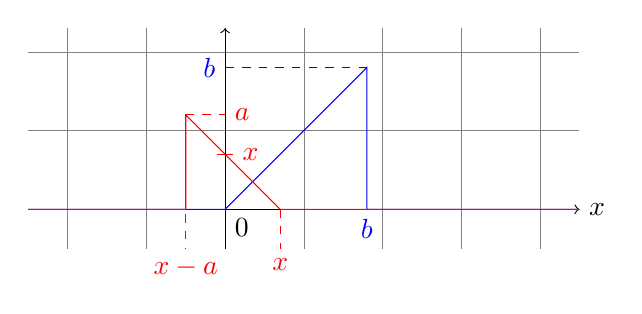
\begin{tikzpicture}
    \GridAxis{-2.5}{4.5}{-0.5}{2.3}
    \begin{scope}[color=blue] % B
        \draw (FuncStart) -- (0,0) -- (1.8,1.8) coordinate(a) |- (FuncEnd);
        \node[below] at (a |- Origin) {$b$};
        \draw[dashed] (a) -- (a -| Origin) node[left] {$b$};
    \end{scope}
    \begin{scope}[color=red] % A
        \draw (FuncStart) -- (-0.5,0) -- +(0,1.2) coordinate(a) -- +(1.2,0) coordinate(b) -- (FuncEnd);
        \draw[dashed] (a) -- (a |- Origin) -- +(0,-0.5) node[below] {$x-a$};
        \draw[dashed] (a) -- (a-| Origin) node[right] {$a$};
        \draw[dashed] (b) -- +(0,-0.5) node[below] {$x$};
        \draw (-0.1,0.7) -- +(0.2,0) node[right] {$x$};
    \end{scope}
\end{tikzpicture}\end{center}
\[
    C_{a,b}(x) =
    \int_0^x (x-t) \times t \times \D t =
    \left[  \frac{xt^2}{2} - \frac{t^3}{3} \right]_0^x =
    \frac{x^3}{6}
\]

\paragraph{Complete inclusion}
$x-a \ge 0 \And x \le b \Equiv x \in [a, b]$.
\begin{center}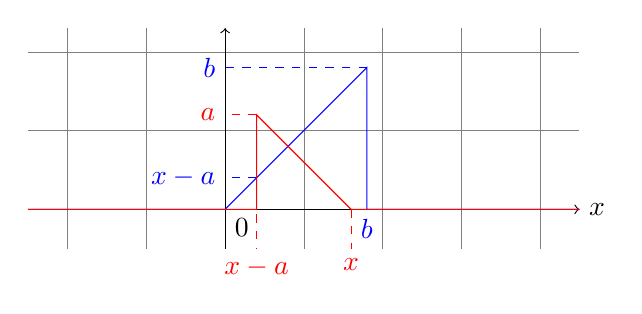
\begin{tikzpicture}
    \GridAxis{-2.5}{4.5}{-0.5}{2.3}
    \begin{scope}[color=blue] % B
        \draw (FuncStart) -- (0,0) -- (1.8,1.8) coordinate(a) |- (FuncEnd);
        \node[below] at (a |- Origin) {$b$};
        \draw[dashed] (a) -- (a -| Origin) node[left] {$b$};
        \draw[dashed] (0.4,0.4) -- (0,0.4) node[left] {$x-a$};
    \end{scope}
    \begin{scope}[color=red] % A
        \draw (FuncStart) -- (0.4,0) -- +(0,1.2) coordinate(a) -- +(1.2,0) coordinate(b) -- (FuncEnd);
        \draw[dashed] (a) -- (a |- Origin) -- +(0,-0.5) node[below] {$x-a$};
        \draw[dashed] (a) -- (a-| Origin) node[left] {$a$};
        \draw[dashed] (b) -- +(0,-0.5) node[below] {$x$};
    \end{scope}
\end{tikzpicture}\end{center}
\[ \begin{split}
    C_{a,b}(x) & = \int_0^a (a-t) \times (t+x-a) \times \D t = \int_0^a (-t^2 +t(2a-x) +a(x-a)) \D t \\
    & =  \left[  -\frac{t^3}{3} + \frac{t^2}{2}(2a-x) +ta(x-a) \right]_0^a = a^2 \left( -\frac{a}{3}+\frac{2a-x}{2}+x-a \right) \\
    & = a^2 \frac{3x-2a}{6}
\end{split} \]

\paragraph{Partial right overlap}
$x-a \le b \And x \ge b \Equiv x \in [b, a+b]$.
\begin{center}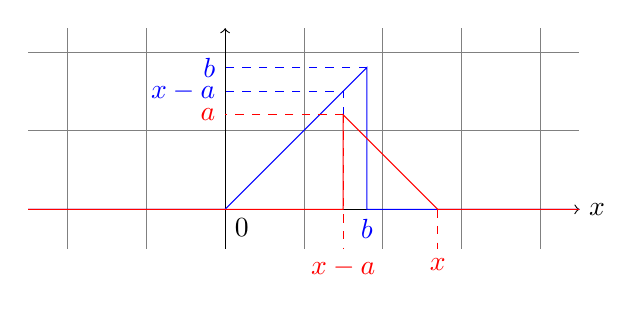
\begin{tikzpicture}
    \GridAxis{-2.5}{4.5}{-0.5}{2.3}
    \begin{scope}[color=blue] % B
        \draw (FuncStart) -- (0,0) -- (1.8,1.8) coordinate(a) |- (FuncEnd);
        \node[below] at (a |- Origin) {$b$};
        \draw[dashed] (a) -- (a -| Origin) node[left] {$b$};
        \draw[dashed] (1.5,1.2) -- (1.5,1.5) -- (0,1.5) node[left] {$x-a$};
    \end{scope}
    \begin{scope}[color=red] % A
        \draw (FuncStart) -- (1.5,0) -- +(0,1.2) coordinate(a) -- +(1.2,0) coordinate(b) -- (FuncEnd);
        \draw[dashed] (a) -- (a |- Origin) -- +(0,-0.5) node[below] {$x-a$};
        \draw[dashed] (a) -- (a-| Origin) node[left] {$a$};
        \draw[dashed] (b) -- +(0,-0.5) node[below] {$x$};
    \end{scope}
\end{tikzpicture}\end{center}
\[ \begin{split}
    C_{a,b}(x) & = \int_0^{a+b-x} (a-t) \times (t+x-a) \times \D t \\
    & = \int_0^{a+b-x} (-t^2 +t(2a-x) +a(x-a)) \D t \\
    & =  \left[  -\frac{t^3}{3} + \frac{t^2}{2}(2a-x) +ta(x-a) \right]_0^{a+b-x} \\
    & =(a+b-x) \left( -\frac{(a+b-x)^2}{3}+\frac{1}{2}(2a-x)(a+b-x)+a(x-a) \right) \\
    & = \frac{1}{6} (a+b-x) (x^2 + x(a+b) -2a^2-2b^2+2ab)
\end{split} \]

\paragraph{No overlap, right}
$x-a \ge b \Equiv x \ge a+b$.
$C_{a,b}(x) = 0$.
\begin{center}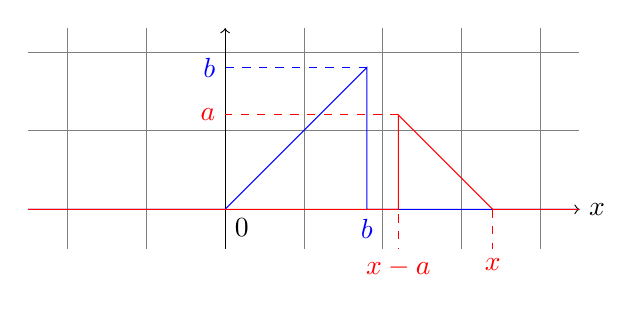
\begin{tikzpicture}
    \GridAxis{-2.5}{4.5}{-0.5}{2.3}
    \begin{scope}[color=blue] % B
        \draw (FuncStart) -- (0,0) -- (1.8,1.8) coordinate(a) |- (FuncEnd);
        \node[below] at (a |- Origin) {$b$};
        \draw[dashed] (a) -- (a -| Origin) node[left] {$b$};
    \end{scope}
    \begin{scope}[color=red] % A
        \draw (FuncStart) -- (2.2,0) -- +(0,1.2) coordinate(a) -- +(1.2,0) coordinate(b) -- (FuncEnd);
        \draw[dashed] (a) -- (a |- Origin) -- +(0,-0.5) node[below] {$x-a$};
        \draw[dashed] (a) -- (a-| Origin) node[left] {$a$};
        \draw[dashed] (b) -- +(0,-0.5) node[below] {$x$};
    \end{scope}
\end{tikzpicture}\end{center}

If we summarize, for $a \le b$:
\[ C_{a,b}(x) = \begin{cases}
    0 & x \le 0 \\
    \frac{x^3}{6} & x \in [0, a] \\
    a^2 \frac{3x-2a}{6} & x \in [a, b] \\
    \frac{1}{6} (a+b-x) (x^2 + x(a+b) -2a^2-2b^2+2ab) & x \in [b, a+b] \\
    0 & x \ge a+b
\end{cases} \]

For any $(a,b)$, using the commutativity of convolution, min/max identities and posing $A=\min(a,b)$ and $B=\max(a,b)$:
\[ C_{a,b}(x) = \begin{cases}
    0 & x \le 0 \\
    \frac{x^3}{6} & x \in [0, A] \\
    A^2 \frac{3x-2A}{6} & x \in [A, B] \\
    \frac{1}{6} (a+b-x) (x^2 + x(a+b) -2a^2-2b^2+2ab) & x \in [B, a+b] \\
    0 & x \ge a+b
\end{cases} \]

%%%%%%%%%%%%%%%%%%%%%%%%%%%%%%%%%%%%%%%%%%%%%%%%%%%%%%%%%%%%%%%%%%%%%%%%%%%%%%%

\end{document}
